\documentclass[a4paper,12pt]{article}
\usepackage{amsmath}
\usepackage{url}
\usepackage{amssymb}
\usepackage{graphicx}
%\documentclass{article}
\usepackage{setspace, enumitem,titlesec}
\usepackage{calc}
			% Activate to display a given date or no date
\usepackage{mathtools}
\usepackage{mathrsfs }
\DeclarePairedDelimiter\ceil{\lceil}{\rceil}
\DeclarePairedDelimiter\floor{\lfloor}{\rfloor}
\usepackage{algorithm}
\usepackage{algorithmic}
\usepackage{fancybox}
%################
\usepackage{float}
\usepackage{makecell}
\usepackage{bbm}
\usepackage{amsmath}
\usepackage{amssymb}
\usepackage{amsthm}
\usepackage{cite}
\usepackage{authblk}
%\usepackage{algpseudocode}

%\renewcommand{\thepseudonum}{\roman{pseudonum}}
\renewcommand\labelenumi{(\theenumi)}
%vector
\renewcommand{\vec}[1]{\mathbf{#1}}
\title {A study of the spherical coordinates parameterization}
%\author{jim.morris.shen@gmail.com}
%\author{The Graduate Center, City University of New York}
\author{Xiaoke Shen}
\affil{the Graduate Center, the City University of New York}
\date{}
\begin{document}
\maketitle

\begin{abstract}
This report provides the results of using the spherical coordinates to resolve the constrained problems.
\end{abstract}
%\textbf{Due Mar 1st 11:59 pm. 10 points for each exercise and 20 points for the extra credit exercise }\\
\part{Introduction}
For the resource allocation problem, suppose resource $p_i$ is allocated to $i$ where $i$ is the index of the object which get the resource, $p_i$ is the allocation ratio to the total available resource. Then we can get:\\
\begin{equation} \label{eq:sum_res_alo}
\sum_{i=1}^{n} p_i = 1
\end{equation}

We can rewrite the equation \ref{eq:sum_res_alo} as bellow:\\
\begin{equation} \label{eq:sum_res_alo_r_2}
\sum_{i=1}^{n} (r_i)^2 = 1
\end{equation}
Any feasible allocation vector $r = (r_1,...,r_n)$ on the unit ball can be described through $n-1$ angels denoted by $\theta_i, 1\leq i \leq n-1$, in the following way. Indeed, the spherical coordinated parameterization of $r$ via $\theta^T = (\theta_1,...,\theta_{n-1}) $ is given by:\\





%\begin{table*}[!ht]
%\begin{center}
%\begin{tabular}{|c|c|c|}
%\hline
%No. & $X_i$ and $n$ of $X_i$&Satisfy requirement of which Theorem\\
%\hline
%1 & \makecell{$X_i \sim \mathcal{N}(0,1)$ \\$n \sim \mathcal{U}\{1,100\} $}& %Theorem 1\\
%\hline
%2 & \makecell{$X_i \sim \mathcal{U}(-1,1)$ or\\ $\mathcal{U}(-10,10)$  with equal chance \\$n \sim \mathcal{U}\{1,100\} $}& Theorem 2\\
%\hline
%\end{tabular}
%\end{center}
%\caption{Experiments for Theorem 1 and Theorem 2. The $\mathcal{U}\{1,100\}$ means  discrete uniform distribution}
%\label{tab:expe12}
%\end{table*}


\part{Experiments}
\section{Cost function is linear}
In this experiment, the cost function is a linear function. The optimization problem is described as below:\\


\begin{equation}\label{eq:1}
\begin{aligned}
\min_{x_1,x_2\in \mathbb{R}} \quad & J(x_1,x_2) = -2x_1-x_2\\
\textrm{s.t.} \quad & 0 \leq x_1 \leq 1\\
              \quad & 0 \leq x_2 \leq 1\\
              \quad & \sum_{i=1}^{2} x_i = 1\\
\end{aligned}
\end{equation}


As $\sum_{i=1}^{2} x_i = 1$, we can change equation \ref{eq:1} to:\\
\begin{equation}\label{eq:2}
\begin{aligned}
\min_{x\in \mathbb{R}} \quad & J(x) = -x-1\\
\textrm{s.t.} \quad & 0 \leq x \leq 1\\
\end{aligned}
\end{equation}


%\begin{equation}
%\begin{aligned}
%\min_{w,b,\xi} \quad & \frac{1}{2}w^{t}w+C\sum_{i=1}^{N}{\xi_{i}}\\
%\textrm{s.t.} \quad & y_{i}(w\phi(x_{i}+b))+\xi_{i}-1\\
%  &\xi\geq0    \\
%\end{aligned}
%\end{equation}



\begin{figure}[H]
\begin{center}
%\fbox{\rule{0pt}{2in} \rule{.9\linewidth}{0pt}}
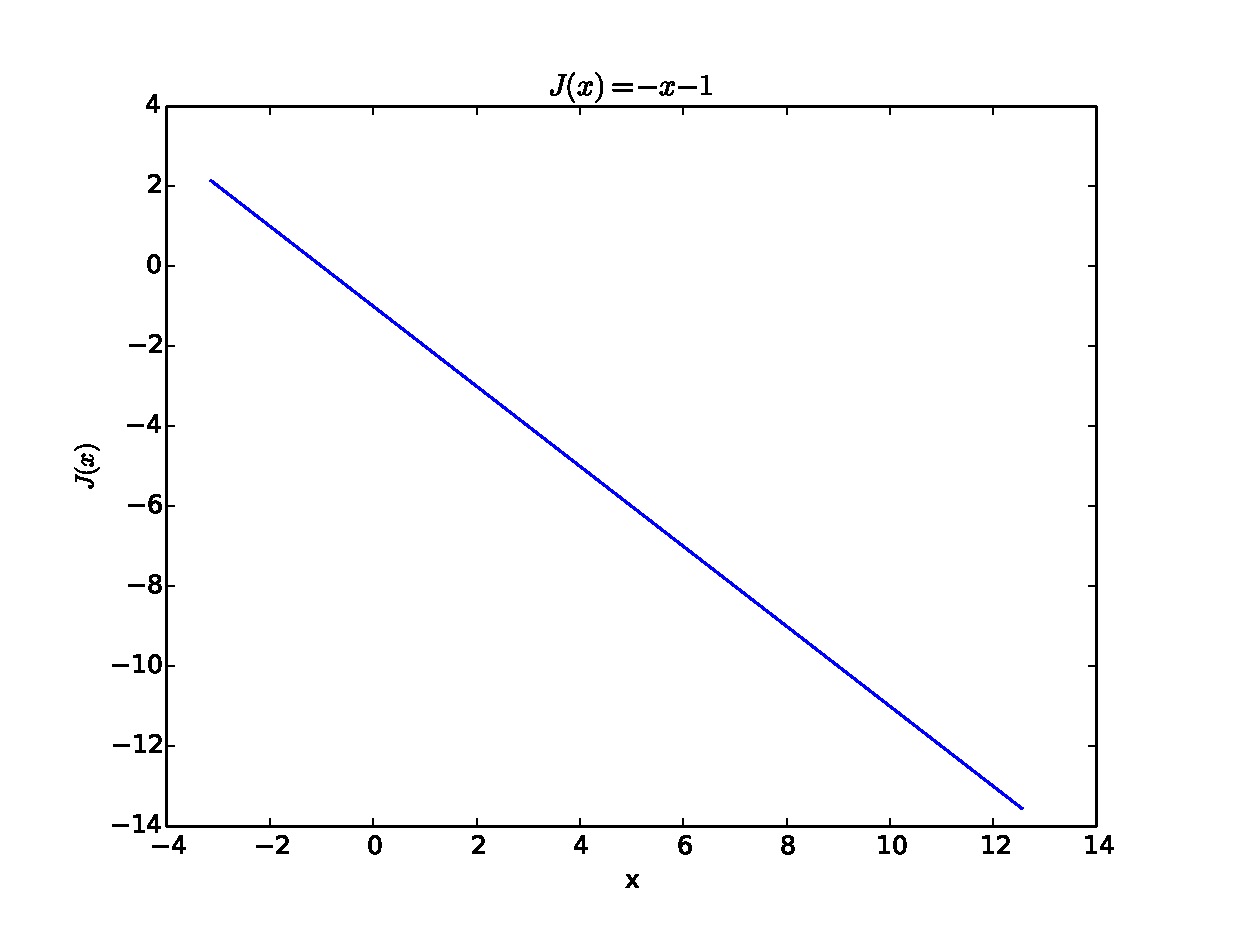
\includegraphics[width=1.0\linewidth]{line.eps}

\end{center}
   \caption{The plot of the cost function: $J(x) = -x-1$.  }
\label{fig:line_cost_sphe}
\end{figure}



\begin{figure}[H]
\begin{center}
%\fbox{\rule{0pt}{2in} \rule{.9\linewidth}{0pt}}
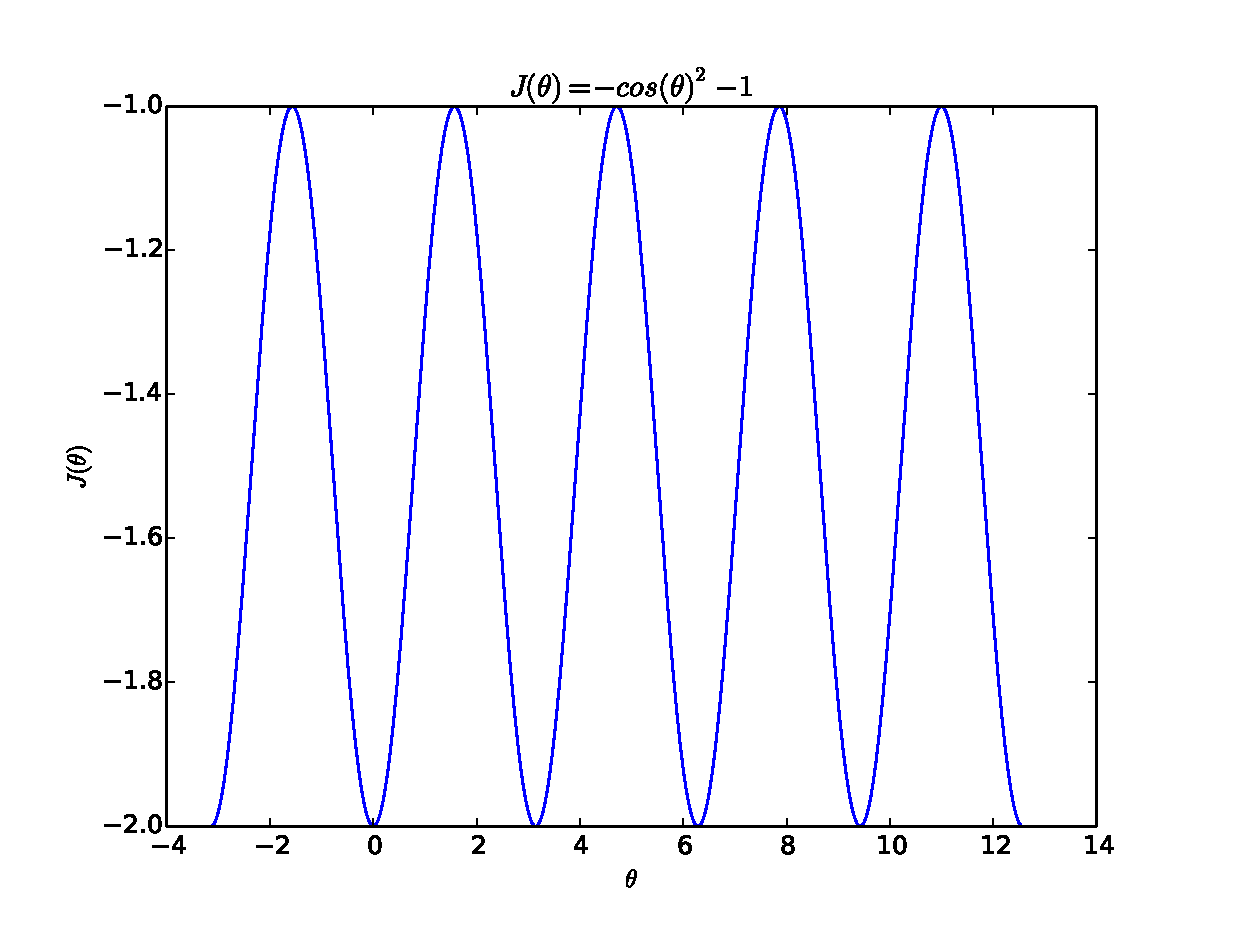
\includegraphics[width=1.0\linewidth]{line_sphe.eps}


\end{center}
   \caption{The plot of the cost function: $J(\theta) = -cos(\theta)^2-1$. }
\label{fig:e1}
\end{figure}



%\begin{table*}[!ht]
%\begin{center}
%\begin{tabular}{|c|c|c|c|c|c|}
%\hline
%thre. $u$&mean &variance&std & Gaussian Parameters&Poisson Parameters \\
%\hline

%1.036 & 522.653 & 322.425& 17.956&$\mu = 522.653, \sigma =17.956$ &$\lambda =522.653 $\\
%1.645 & 194.570 & 168.123& 12.966&$\mu = 194.570, \sigma =12.966$ &$\lambda =194.570 $\\
%2.000 & 91.139 & 86.115& 9.280&$\mu = 91.139, \sigma =9.280$ &$\lambda =91.139 $\\
%2.800 & 10.440 & 10.228& 3.198&$\mu = 10.440, \sigma =3.198$ &$\lambda =10.440 $\\

%\hline
%\end{tabular}
%\end{center}
%\caption{Statistic results and empirical disturibution parameters of $\mathbf{K}$ when the threshold $m=4096$}
%\label{tab:k}
%\end{table*}




\bibliography{jimmy_shen}
\bibliographystyle{ieeetr}
  
 \end{document}
